\chapter{Introducción}
\label{cap:capitulo1}
\setcounter{page}{1}

La tarea Sigue-Personas es una de las más empleadas y solicitadas en los Robots de Servicio para multitud de sectores que incorporan soluciones robóticas. El siguiente TFG propone desarrollar dos nuevos ejercicios para Unibotics con el objetivo de que los usuarios programen un robot Turtlebot2 tanto en simulado como en real para que realice dicha tarea.\\

Este primer capítulo trata de presentar el estado actual de varios campos de la Robótica que están directamente relacionados con este proyecto para poner en contexto al lector y faciitar su lectura.\\

Por un lado presentaremos la Robótica Móvil, un sector de la robótica que está en constante crecimiento y muy presente en la Robótica de Servicio; por otra parte, introduciremos las Redes Neuronales, un avance significativo en IA que ha permitido realizar aplicaciones muy robustas basadas en la percepción y el razonamiento; y por último hablaremos de la Robótica Educativa, e introduciremos varias plataformas como TheConstruct, Robotics Academy, o Unibotics siendo estas dos últimas las que incorporarán el ejercicio educativo Sigue-Persona.

\section{Robótica Móvil}
\label{sec:robotica_movil}

La robótica es la ciencia que engloba varias ramas tecnológicas o disciplinas, con el objetivo de diseñar máquinas (``robots'') que sean capaces de realizar tareas automatizadas o de simular el comportamiento humano o animal, en función de la capacidad de su software. \cite{revistaderobots}\\

La robótica se ve impulsada a partir de 1952 con la primera máquina de control numérico del MIT que era capaz de automatizar algunas tareas industriales. En 1961, la compañía Unimates introdujo el primer robot industral en la General Motors, y, 5 años después, comenzó el desarrollo del primer robot móvil llamado Shakey [Nilsson, 1984].\\

\begin{figure} [h!]
  \begin{center}
    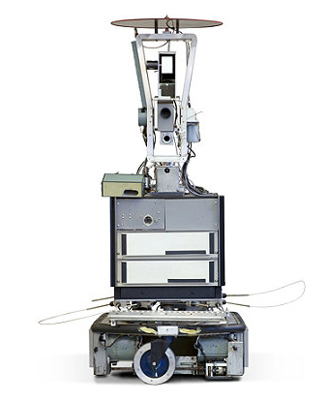
\includegraphics[width=5cm]{imagenes/shakey.jpg}
  \end{center}
  \caption{Shakey (1966-1972) \cite{shakey-the-robot}}
  \label{fig:shakey}
\end{figure}\

Un robot móvil es aquel robot capaz de desplazarse mediante ruedas o patas sobre su entorno.

\section{Redes Neuronales}
\label{sec:redes_neuronales}

Según \emph{Arthur Samuel}, el Aprendizaje Automático o Machine Learning es el ``campo de estudio que otorga a los ordenadores la capacidad de aprender sin ser programados explícitamente''. En nuestro campo, la robótica, un robot puede conseguir un objetivo a través de un modelo computacional que le ha permitido ``aprender'' a maximizar el rendimiento de la tarea encomendada. Un ejemplo puede ser un coche autónomo que aparca sólo gracias a un complejo entrenamiento previo que le ha \emph{enseñado} a realizar dicha tarea.\\

Las Redes Neuronales son un modelo computacional inspirado en el cerebro humano. Se usa tanto en problemas de Aprendizaje Supervisado como no Supervisado. Típicamente se trata de un conjunto de capas formado por varias neuronas que se encuentran interconectadas. Suelen dividirse en 1 capa de entrada, 1 o más capas ocultas y 1 capa de salida.\\

En la capa de entrada las neuronas reciben el valor de las características del problema a clasificar y se combina con un valor de pesos precalculado. A través de las capas ocultas, se realizan varios cálculos dependiendo del tamaño de la red y, por último, en la capa de salida se retorna el valor o valores que la red neuronal considera que puede ser la solución al problema (por ejemplo: El objeto que hay encima de la mesa es un libro).\\

Pero para entender las Redes Neuronales primero hay que comprender la unidad mínima de una Red: \textbf{El Perceptrón}\\

\section{Educación en Robótica}
\label{sec:educacion_robotica}

\subsection{TheConstruct}
\label{sec:the_construct}

\subsection{Robotics Academy}
\label{sec:robotics_academy}

\subsection{Unibotics}
\label{sec:unibotics}


